\section{Bayesian Optimization}
\begin{framed}
    The \textbf{Regret} for a time horizon $T$ associated with choices $\{\vx_t\}_{t=1}^T$ is defined as: $R_T \defeq \sum_{t=1}^T \underbrace{\left({\max_\vx \opt{f}(\vx) - \opt{f}(\vx_t)}\right)}_{\text{\textit{instantaneous regret}}}$.
\end{framed}
Goal: Achieve sublinear regret: $\lim_{T\to\infty} \frac{R_T}{T} = 0$.
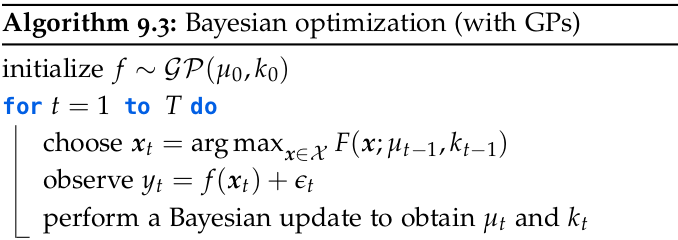
\includegraphics[width=0.98\linewidth]{images/Bayesian_Optimization.png}
$F$: \textbf{acquisition function} \\
\textbf{Upper confidence bound}: \\$\vx_{t+1} \defeq \argmax_{\vx \in \spX} \mu_{t}(\vx) + \beta_{t+1} \sigma_{t}(\vx)$, where $\sigma_t(\vx) \defeq \sqrt{k_t(\vx, \vx)}$. If $\beta_t = 0$ then UCB is purely exploitative; if $\beta_t \to \infty$, UCB recovers uncertainty sampling.
\begin{framed}
    Choosing $\beta_t$ appropriately we get: $R_T = \BigO{\sqrt{T \gamma_T}}$, where \\
    $\gamma_T \defeq \max_{\substack{\sS \subseteq \spX \\ |\sS| = T}} \underbrace{\frac{1}{2} \log\det{\mI + \sigman^{-2} \mK_{\sS\sS}}}_{\I{\vf_\sS}{\vy_\sS}}$ \\
    max. information gain after $T$ rounds.
\end{framed}
\begin{framed}
    \textbf{Information gain of some kernels}: \\
    Linear: $\gamma_T = \BigO{d ~\log T}$ \\
    Gaussian: $\gamma_T = \BigO{(\log T)^{d+1}}$ \\
    Matérn for $\nu > \frac{1}{2}$: $\gamma_T = \BigO{T^{\frac{d}{2\nu + d}} (\log T)^{\frac{2\nu}{2\nu + d}}}$ \\
    which are sublinear $\Rightarrow$ sublinear regret.
\end{framed}
\textbf{Thompson Sampling}: Sample a function $\Tilde{f}_{t+1} \sim p(\cdot \mid \vx_{1:t}, y_{1:t})$ from posterior dist.
Then maximize $\Tilde{f}_{t+1}$, $\vx_{t+1} \defeq \argmax_{\vx \in \spX} \Tilde{f}_{t+1}(\vx)$.
